\documentclass[12pt]{beamer}
\usepackage[utf8]{inputenc}
\graphicspath{{Imagenes/}{../Imagenes/}}
%\usepackage[latin1]{inputenc}
\usepackage[spanish]{babel}
%\usetheme{Warsaw}
%\usepackage{euler}
\usepackage{amsmath}
\usepackage{amsthm}
%\usepackage[table]{xcolor}
\usepackage{booktabs}
\usepackage{tabulary}
\usepackage{nccmath}
\usepackage{multicol}
\usepackage{multirow}
\usepackage{graphicx}
\usepackage{color,colortbl}
\usepackage{hhline}
\usepackage{listings}
\usepackage{tikz}
\usetikzlibrary{decorations.markings}
% Introduce a new counter for counting the nodes needed for circling
\newcounter{nodecount}
% Command for making a new node and naming it according to the nodecount counter
\newcommand\tabnode[1]{\addtocounter{nodecount}{1} \tikz \node (\arabic{nodecount}) {#1};}

% Some options common to all the nodes and paths
\tikzstyle{every picture}+=[remember picture,baseline]
\tikzstyle{every node}+=[inner sep=0pt,anchor=base,
minimum width=2.2cm,align=center,text depth=.15ex,outer sep=1.5pt]
\tikzstyle{every path}+=[thick, rounded corners]
\renewcommand*{\multirowsetup}{\centering}
\lstset{ %
language=Python,                % choose the language of the code
basicstyle=\small,       % the size of the fonts that are used for the code
numbers=left,                   % where to put the line-numbers
numberstyle=\footnotesize,      % the size of the fonts that are used for the line-numbers
stepnumber=1,                   % the step between two line-numbers. If it is 1 each line will be numbered
numbersep=5pt,                  % how far the line-numbers are from the code
backgroundcolor=\color{white},  % choose the background color. You must add \usepackage{color}
showspaces=false,               % show spaces adding particular underscores
showstringspaces=false,         % underline spaces within strings
showtabs=false,                 % show tabs within strings adding particular underscores
frame=single,   		% adds a frame around the code
tabsize=4,  		% sets default tabsize to 2 spaces
captionpos=b,   		% sets the caption-position to bottom
breaklines=true,    	% sets automatic line breaking
breakatwhitespace=false,    % sets if automatic breaks should only happen at whitespace
escapeinside={\#}{)}          % if you want to add a comment within your code
}
%\usepackage{epstopdf}
\DeclareGraphicsExtensions{.pdf,.png,.jpg}
\renewcommand {\arraystretch}{1.5}
\mode<presentation>
{
  \usetheme{Warsaw}
  \setbeamertemplate{headline}{}
  \setbeamercovered{invisible}
%  \setbeamercovered{transparent}
  % or whatever (possibly just delete it)
}

%\documentclass[12pt]{beamer}
\newenvironment{ConCodigo}[1]
  {\begin{frame}[fragile,environment=ConCodigo]{#1}}
  {\end{frame}}
\graphicspath{{Imagenes/}{../Imagenes/}}
\usepackage[utf8]{inputenc}
\usepackage[spanish]{babel}
\usepackage{hyperref}
\usepackage{etex}
\reserveinserts{28}
\usepackage{amsmath}
\usepackage{amsthm}
\usepackage{mathtools}
\usepackage{multicol}
\usepackage{multirow}
\usepackage{tabulary}
%\usepackage{tabularx}
\usepackage{booktabs}
\usepackage{nccmath}
\usepackage{biblatex}
\usepackage{epstopdf}
\usepackage{graphicx}
\usepackage{siunitx}
\sisetup{scientific-notation=true}
%\usepackage{fontspec}
\usepackage{lmodern}
\usepackage{float}
\usepackage[format=hang, font=footnotesize, labelformat=parens]{caption}
\usepackage[autostyle,spanish=mexican]{csquotes}
\usepackage{standalone}
\usepackage{tikz}
\usepackage[siunitx]{circuitikz}
\usetikzlibrary{arrows,patterns,shapes}
\usetikzlibrary{decorations.markings}
\usetikzlibrary{arrows}
\usepackage{color}
%\usepackage{beton}
%\usepackage{euler}
%\usepackage[T1]{fontenc}
\usepackage[sfdefault]{roboto}  %% Option 'sfdefault' only if the base font of the document is to be sans serif
\usepackage[T1]{fontenc}
\renewcommand*\familydefault{\sfdefault}
\DeclareGraphicsExtensions{.pdf,.png,.jpg}
\usepackage{hyperref}
\renewcommand {\arraystretch}{1.5}
\newcommand{\python}{\texttt{python}}
\usefonttheme[onlymath]{serif}
\setbeamertemplate{navigation symbols}{}
\usetikzlibrary{patterns}
\usetikzlibrary{decorations.markings}
\tikzstyle{every picture}+=[remember picture,baseline]
%\tikzstyle{every node}+=[inner sep=0pt,anchor=base,
%minimum width=2.2cm,align=center,text depth=.15ex,outer sep=1.5pt]
%\tikzstyle{every path}+=[thick, rounded corners]
\setbeamertemplate{caption}[numbered]
\newcommand{\ptm}{\fontfamily{ptm}\selectfont}
%Se usa la plantilla Warsaw modificada con spruce
\mode<presentation>
{
  \usetheme{Warsaw}
  \setbeamertemplate{headline}{}
  \useoutertheme{default}
  \usecolortheme{beaver}
  \setbeamercovered{invisible}
}
\AtBeginSection[]
{
\begin{frame}<beamer>{Contenido}
\normalfont\mdseries
\tableofcontents[currentsection]
\end{frame}
}

%\usepackage{listings}
\lstset{ %
language=Python,                % choose the language of the code
basicstyle=\small,       % the size of the fonts that are used for the code
numbers=left,                   % where to put the line-numbers
numberstyle=\small,      % the size of the fonts that are used for the line-numbers
stepnumber=1,                   % the step between two line-numbers. If it is 1 each line will be numbered
numbersep=5pt,                  % how far the line-numbers are from the code
backgroundcolor=\color{white},  % choose the background color. You must add \usepackage{color}
showspaces=false,               % show spaces adding particular underscores
showstringspaces=false,         % underline spaces within strings
showtabs=false,                 % show tabs within strings adding particular underscores
frame=single,   		% adds a frame around the code
tabsize=2,  		% sets default tabsize to 2 spaces
captionpos=b,   		% sets the caption-position to bottom
breaklines=true,    	% sets automatic line breaking
breakatwhitespace=false,    % sets if automatic breaks should only happen at whitespace
escapeinside={\%},          % if you want to add a comment within your code
stringstyle =\color{magenta},
keywordstyle = \color{blue},
commentstyle = \color{green},
identifierstyle = \color{red}
}
\title{Tema 2 - Operaciones matem\'{a}ticas b\'{a}sicas}
\subtitle{C\'{a}lculo de ra\'{i}ces}
%\subsubtitle{Curso de F\'{i}sica Computacional}
\author{M. en C. Gustavo Contreras May\'{e}n}
%\date{18 de septiembre de 2012}
%\email{curso.fisica.comp@gmail.com}
%\ptsize{10}
\begin{document}
\maketitle
\fontsize{14}{14}\selectfont
\spanishdecimal{.}
\begin{frame}{Contenido}
\tableofcontents[pausesections]
\end{frame}
\section{C\'{a}lculo de ra\'{i}ces}
\begin{frame}
\frametitle{C\'{a}lculo de ra\'{i}ces}
Sea $y= f(x)$.  Los valores de $x$ que hacen que $y=0$ se
denominan \textcolor{blue}{ra\'{i}ces de la ecuaci\'{o}n}.
\\
\bigskip
El teorema fundamental del \'{a}lgebra indica que todo polinomio de grado $n$, tiene $n$ ra\'{i}ces. En el caso de las ra\'{i}ces reales, se tiene que corresponden a los valores $x$ que hacen que la funci\'{o}n corte el eje de las abscisas:
\end{frame}
\begin{frame}
\frametitle{Ejemplo de la funci\'{o}n seno(x)}
\begin{figure}
	\centering
	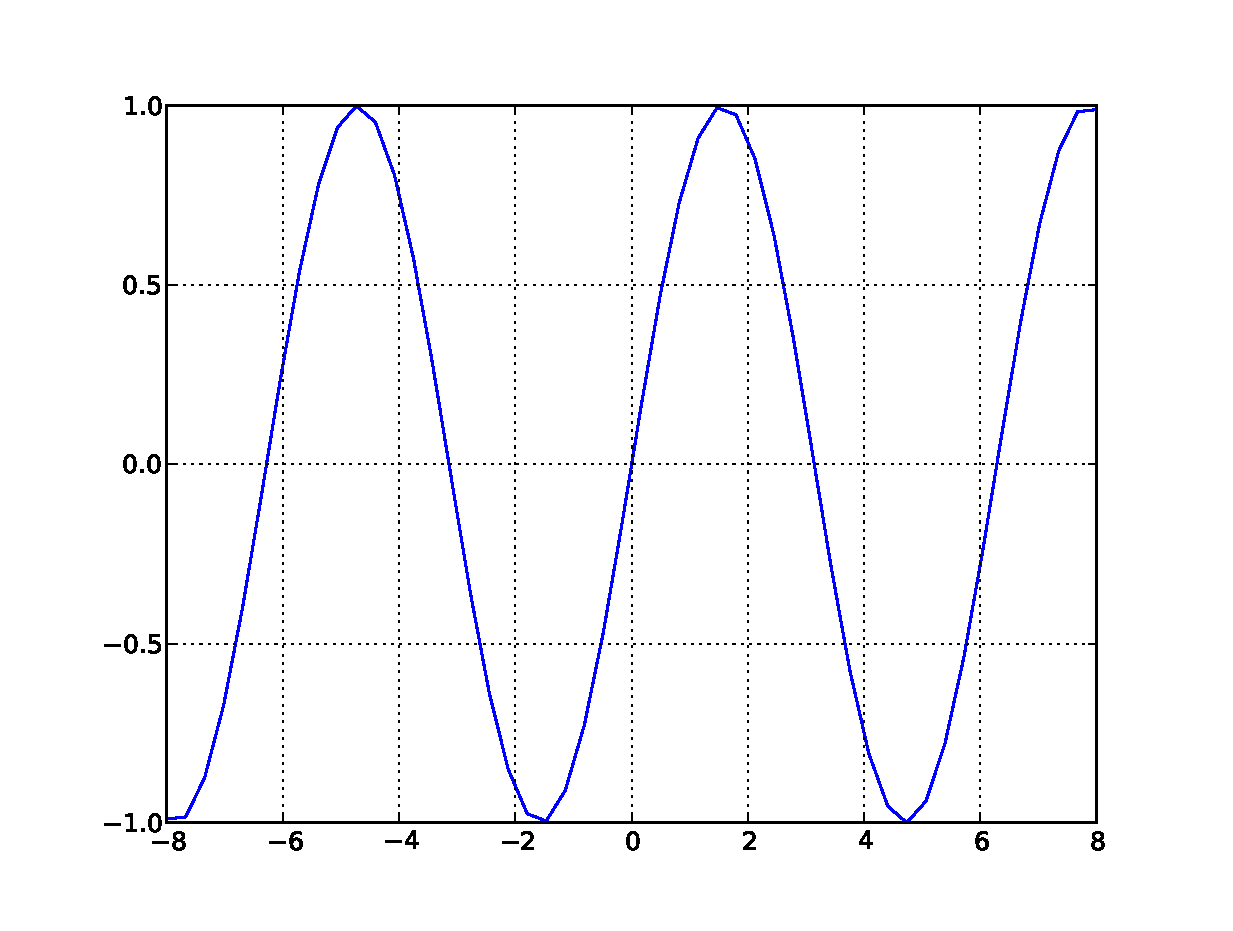
\includegraphics[scale=0.4]{raices00.eps} 
\end{figure}
\end{frame}
\begin{frame}
Las ra\'{i}ces de un polinomio pueden ser reales o complejas.
\\
\bigskip
Si un polinomio tiene coeficientes reales
\[ a_{0},a_{1},a_{2},\ldots,a_{n-1},a_{n} \]
entonces todas las ra\'{i}ces complejas siempre ocurrir\'{a}n en pares conjugados complejos.
\end{frame}
\begin{frame}
Por ejemplo, un polinomio c\'{u}bico tiene la siguiente
forma general:
\[ f(x)= a_{0}x^{3}+a_{1}x^{2}+a_{2}x+a_{3}\]
\begin{enumerate}
\item Tres ra\'{i}ces reales distintas.
\item Una ra\'{i}z real con multiplicidad 3.
\item Una ra\'{i}z real simple y una ra\'{i}z real con multiplicidad 2.
\item Una ra\'{i}z real y un par conjugado complejo.
\end{enumerate}
\end{frame}
\begin{frame}[fragile]
\frametitle{Tres ra\'{i}ces distintas}
\begin{minipage}{5cm}
\fontsize{12}{12}\selectfont
\[ \begin{split}
f(x)=& x^{3} - 3x^{2}-x+3 \\
=& (x-3)(x+1)(x-1)
\end{split} \]
Las ra\'{i}ces son:
\[ \begin{split}
x_{1} =& 3 \\
x_{2} =& -1 \\
x_{3} =& 1 \\
\end{split}\]
\end{minipage}
\hspace{0.5cm}
\begin{minipage}{4.5cm}
\begin{figure}
	\centering
	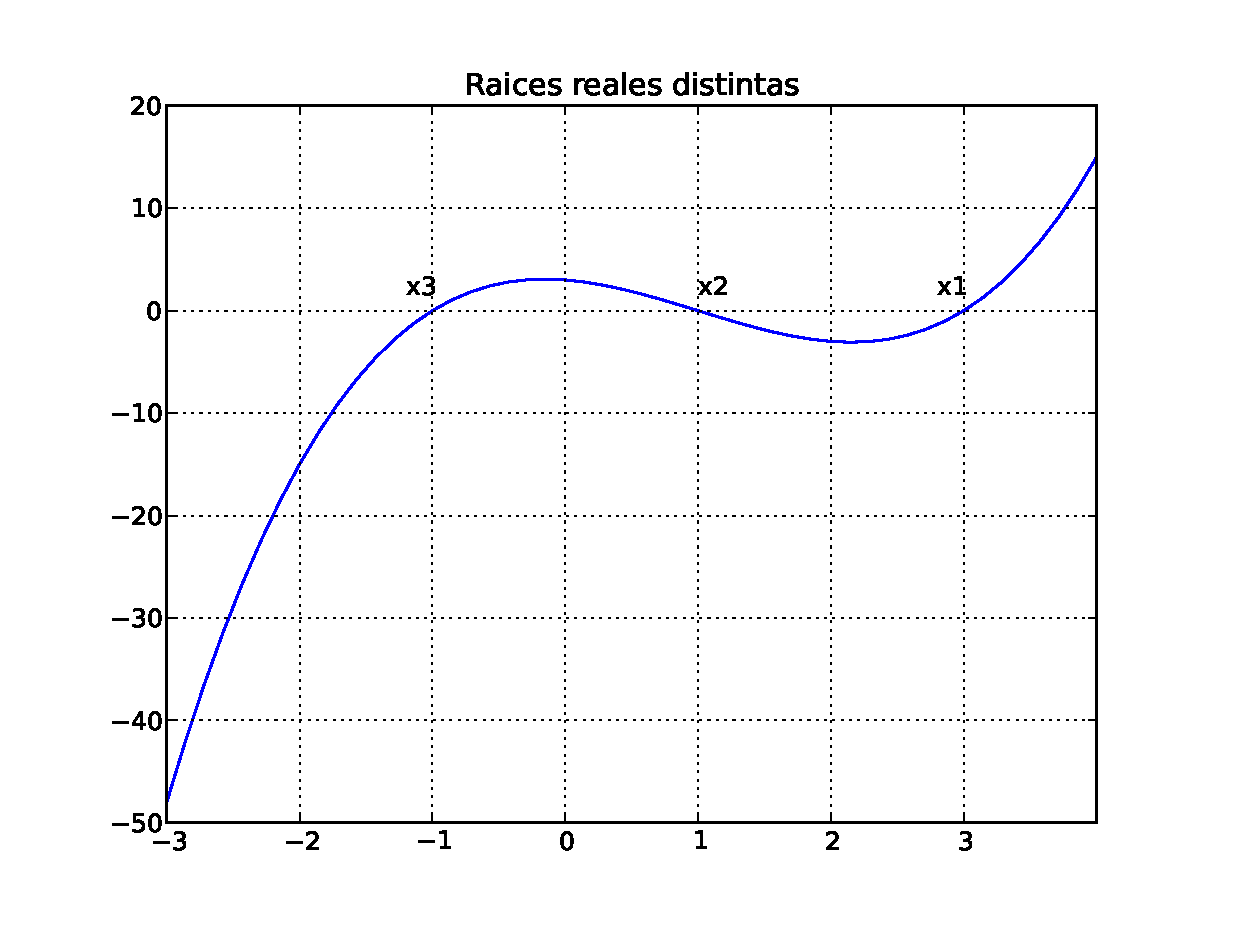
\includegraphics[scale=0.3]{raices01.eps} 
\end{figure}
\end{minipage}
\end{frame}
\begin{frame}[fragile]
\frametitle{Ra\'{i}z real con multiplicidad 3}
\begin{minipage}{5cm}
\fontsize{12}{12}\selectfont
\[ \begin{split}
f(x)=& x^{3} - 6x^{2} + 12x - 8 \\
=& (x-2)^{3}
\end{split} \]
Las ra\'{i}ces son:
\[ \begin{split}
x_{1} =& 2 \\
x_{2} =& 2 \\
x_{3} =& 2 \\
\end{split}\]
\end{minipage}
\hspace{0.5cm}
\begin{minipage}{4.5cm}
\begin{figure}
	\centering
	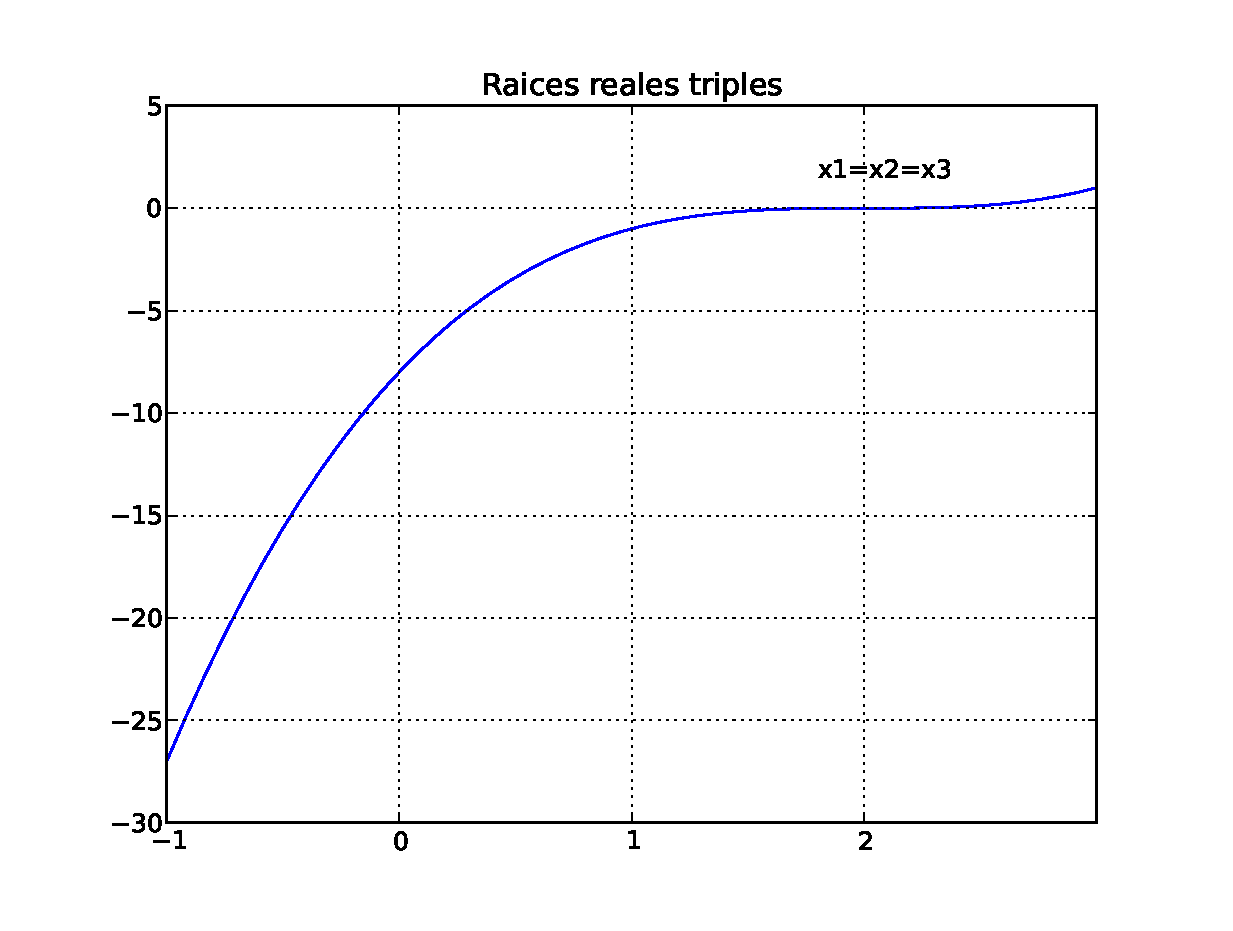
\includegraphics[scale=0.3]{raices02.eps} 
\end{figure}
\end{minipage}
\end{frame}
\begin{frame}[fragile]
\frametitle{Ra\'{i}z real simple y \\ una ra\'{i}z real con multiplicidad 2}
\begin{minipage}{5cm}
\fontsize{12}{12}\selectfont
\[ \begin{split}
f(x)=& x^{3} - 12x + 16 \\
=& (x+4)(x-2)^{2}
\end{split} \]
Las ra\'{i}ces son:
\[ \begin{split}
x_{1} =& -4 \\
x_{2} =& 2 \\
x_{3} =& 2 \\
\end{split}\]
\end{minipage}
\hspace{0.5cm}
\begin{minipage}{4.5cm}
\begin{figure}
	\centering
	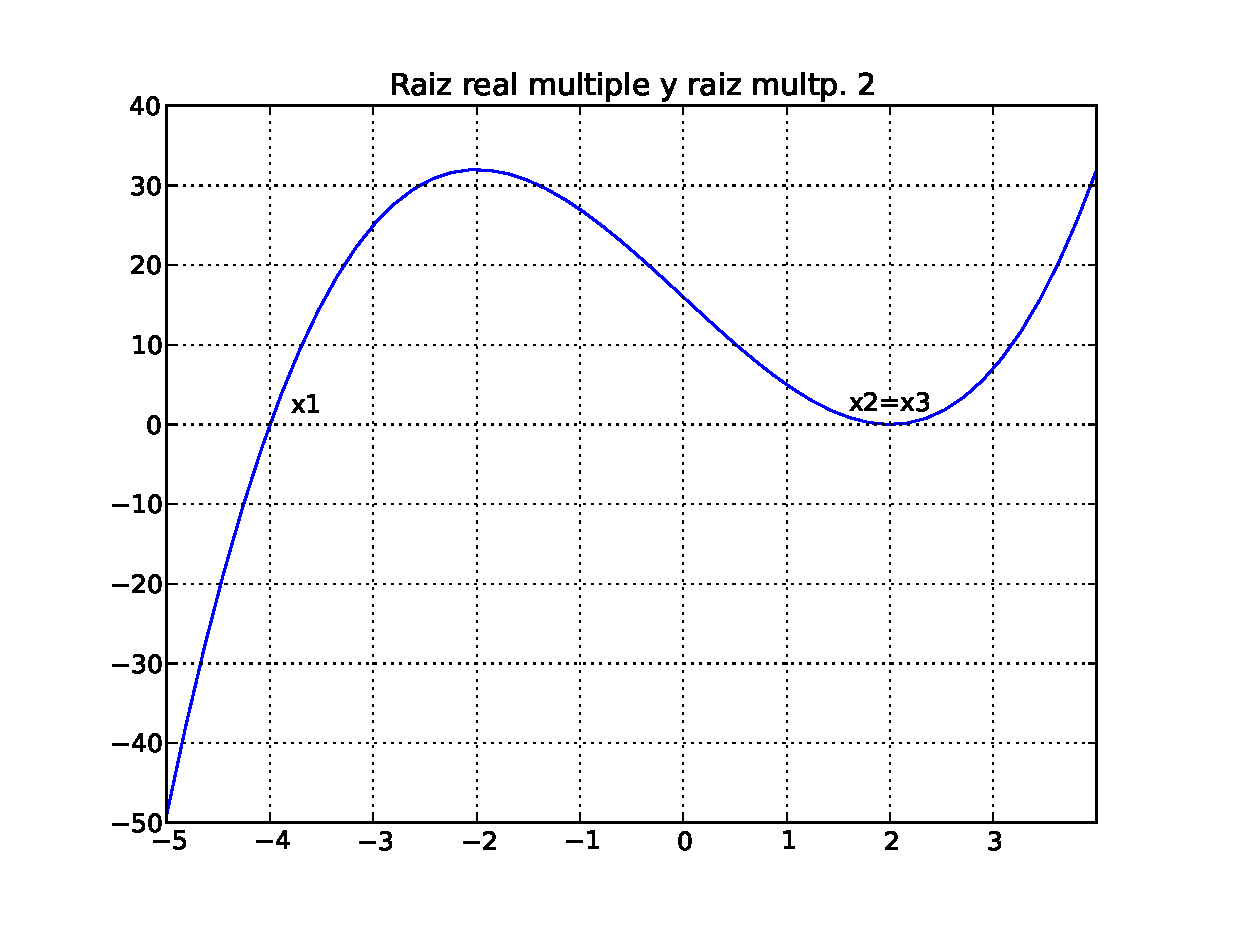
\includegraphics[scale=0.3]{raices03.eps} 
\end{figure}
\end{minipage}
\end{frame}
\begin{frame}[fragile]
\frametitle{Ra\'{i}z real y un par conjugado complejo}
\begin{minipage}{5cm}
\fontsize{12}{12}\selectfont
\[ \begin{split}
f(x)=& x^{3} - 2x^{2}- 3x +10  \\
=& (x+2)(x- (2+i))* {}\\
*& (x-(2-i))
\end{split} \]
Las ra\'{i}ces son:
\[ \begin{split}
x_{1} =& -2 \\
x_{2} =& 2+i \\
x_{3} =& 2-i \\
\end{split}\]
\end{minipage}
\hspace{0.5cm}
\begin{minipage}{4.5cm}
\begin{figure}
	\centering
	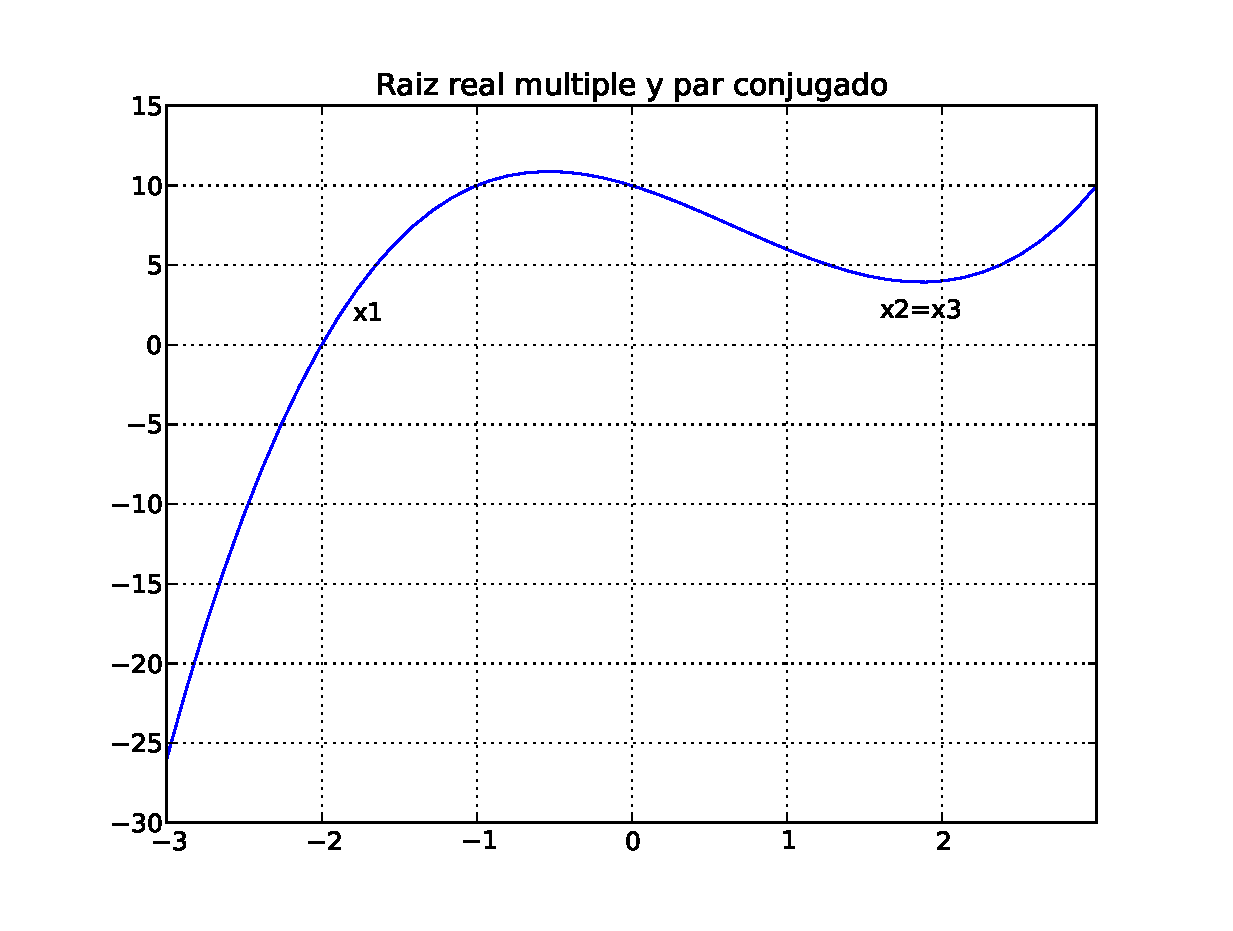
\includegraphics[scale=0.3]{raices04.eps} 
\end{figure}
\end{minipage}
\end{frame}
\section{Funciones algebraicas}
\begin{frame}
\frametitle{Funciones algebraicas}
Sea $g=f(x)$ la funci\'{o}n expresada como
\[ f_{n}y^{n} + f_{n-1}y^{n-1} + \ldots + f_{1}y + f_{0} = 0 \]
Donde $f_{i}$ es un polinomio de orden $i$ en $x$.
\\
\bigskip
Los polinomios son un caso simple de funciones algebraicas que se representan generalmente como
\[f_{n}(x) = a_{0} + a_{1}x + a_{2} x^{2}+ \ldots +a_{n}x^{n} \]
Donde $n$ es el orden del polinomio.
\end{frame}
\section{Funciones trascendentales}
\begin{frame}
\frametitle{Funciones trascedentales}
Son aquellas que no son algebraicas.
\\
\bigskip
Comprenden a las funciones trigonom\'{e}tricas, exponenciales, logar\'{i}tmicas, entre otras.
\\
\bigskip
Ejemplos:
\begin{itemize}
\item \[ f(x)=ln(x^{2}-1) \]
\item \[g(x)=e^{-0.2x} \sin(3x-5) \]
\end{itemize}
\end{frame}
\begin{frame}
Los m\'{e}todos num\'{e}ricos est\'{a}ndar para encontrar
ra\'{i}ces pueden clasificarse en dos rubros:
\\
\bigskip
\textbf{1.} La determinaci\'{o}n de las ra\'{i}ces reales de ecuaciones algebraicas y trascendentales. Las t\'{e}cnicas a emplear en estos casos se diseñaron con el fin de encontrar el valor de una ra\'{i}z simple de acuerdo con un conocimiento previo de su posici\'{o}n aproximada.
\end{frame}
\begin{frame}
\textbf{2.} La determinaci\'{o}n de todas las raíces reales y complejas de un polinomio, para lo cual los m\'{e}todos num\'{e}ricos est\'{e}n diseñados espec\'{i}ficamente para polinomios. 
\\
\bigskip
Determinan sistem\'{a}ticamente todas las ra\'{i}ces del polinomio en lugar de hacerlo s\'{o}lo con una, dada la posición aproximada.
\end{frame}
\section{M\'{e}todo de incrementos sucesivos}
\begin{frame}
\frametitle{M\'{e}todo de incrementos sucesivos}
Podemos aproximar mucho mejor las ra\'{i}ces de una funci\'{o}n, cuando la graficamos.
\\
\bigskip
Con una gr\'{a}fica general de unos cuantos puntos, tendr\'{i}amos lo necesario para considerar los valores de las ra\'{i}ces.
\\
\bigskip
El m\'{e}todo de b\'{u}squeda incremental es una herramienta \'{u}til que podemos adoptar en conjunto con otras estrategias de c\'{a}lculo de ra\'{i}ces, por s\'{i} s\'{o}lo, \'{e}ste m\'{e}todo no nos ofrece m\'{a}s que una referencia sobre en d\'{o}nde podr\'{i}an estar esas ra\'{i}ces.
\end{frame}
\begin{frame}
La idea b\'{a}sica detr\'{a}s del m\'{e}todo de b\'{u}squeda incremental es simple: si $f(x_{1})$ y $f(x_{2})$ tienen signos opuestos, entonces hay al menos una ra\'{i}z en el intervalo $(x_{1}, x_{2})$.
\end{frame}
\begin{frame}[fragile]
\frametitle{Caso en donde es posible encontrar la ra\'{i}z}
\begin{center}
	\begin{tikzpicture}[font=\footnotesize, scale=1.3]
		\draw[<->](0,0) -- (6,0);
		\draw[<->](3,-2) -- (3,2);
		\draw [red] (0.5,1.5) .. controls (2,0.2) and (4,-1) .. (5.5,-1.5);
		\draw[dashed] (1,0) -- (1,1.1);
		\draw (0.9,-0.2) node {a}; 
		\draw (1.2,1.4) node {f(a)};
		\draw[dashed] (5,0) -- (5,-1.33);
		\draw (5,0.2) node {b}; 
		\draw (5,-1.7) node {f(b)};
		\draw(4.5,1.5) node {$f(a)*f(b)<0$};
	\end{tikzpicture}
\end{center}
\end{frame}
\begin{frame}
\frametitle{Caso en donde no es posible encontrar la ra\'{i}z}
\begin{center}
	\begin{tikzpicture}[font=\footnotesize, scale=1.3]
		\draw[<->](0,0) -- (6,0);
		\draw[<->](3,-1) -- (3,3);
		\draw [red] (0.5,2.5) .. controls (2.5,0.5) and (3.5,0.5) .. (5.5,2.5);
		\draw [dashed] (1,0) -- (1,2.1);
		\draw (1,-0.2) node {a};
		\draw (1.1,2.2) node {f(a)};
		\draw [dashed] (4.5,0) -- (4.5,1.65);
		\draw (4.5,-0.2) node {b};
		\draw (4.5, 2) node {f(b)};
		\draw (5,3.5) node {$f(a)*f(b)>0$};
	\end{tikzpicture}
\end{center}
\end{frame}
\begin{frame}
Si el intervalo es lo suficientemente pequeño, es probable que contenga una sola ra\'{i}z. As\'{i}, los ceros de $f(x)$ puede ser detectados mediante la evaluaci\'{o}n de la funci\'{o}n a intervalos $\Delta x$ y mirando cuando se presente un cambio de signo en la funci\'{o}n.
\end{frame}
\begin{frame}
Hay varios problemas con el m\'{e}todo de b\'{u}squeda incremental:
\begin{enumerate}
\item Es posible perder dos ra\'{i}ces muy pr\'{o}ximas entre s\'{i}, si el incremento de búsqueda $\Delta x$ es mayor que la separaci\'{o}n de las ra\'{i}ces.
\item Una ra\'{i}z doble (dos ra\'{i}ces que coinciden) no ser\'{a} detectada.
\item Algunas singularidades de $f(x)$ se puede confundir con ra\'{i}ces. Por ejemplo, $f(x) = \tan x$. Tiene cambios de signo en $x = \pm 1/2 n\pi$ con $n = 1, 3, 5,\ldots$
\end{enumerate}
\end{frame}
\begin{frame}
Estos puntos no son ceros verdaderos, ya que la funci\'{o}n no cruza el eje $x$.
\begin{figure}
	\centering
	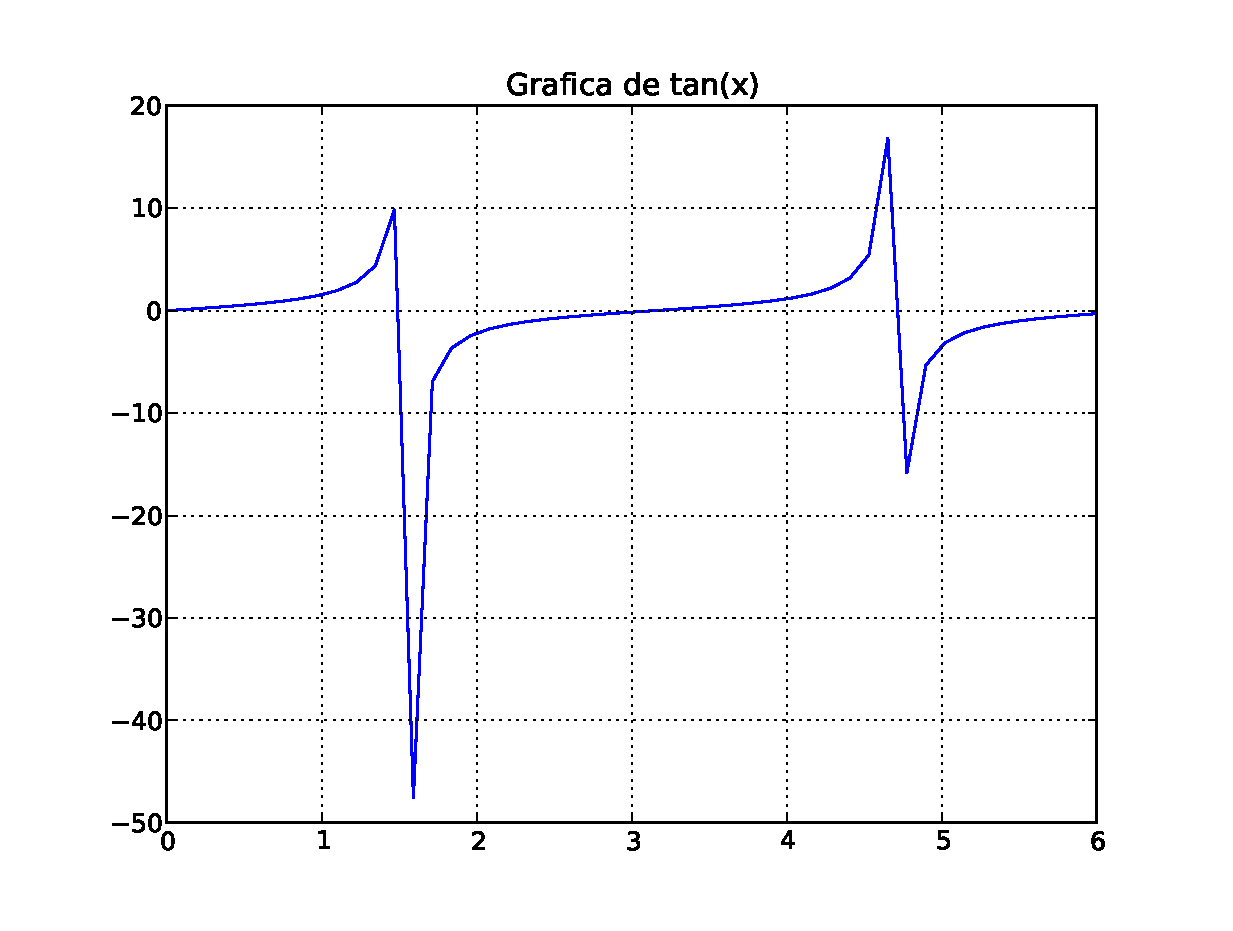
\includegraphics[scale=0.4]{raices05.eps} 
\end{figure}
\end{frame}
\subsection{C\'{o}digo M\'{e}todo de incrementos sucesivos}
\begin{frame}
\frametitle{C\'{o}digo M\'{e}todo de incrementos sucesivos}
El c\'{o}digo busca un cero de la función $f$ que proporciona el usuario en el intervalo
$(a,b)$ en incrementos de $dx$.
\\
\bigskip
Se devuelve el intervalo $(x_{1}, x_{2})$ donde se encuentra la ra\'{i}z, si la b\'{u}squeda
se ha realizado correctamente; se devuelve $x_{1} = x_{2} = \mathsf{None}$ cuando no se encontraron ra\'{i}ces.
\end{frame}
\begin{frame}
Luego de que se encontr\'{o} la primera ra\'{i}z, (la m\'{a}s cercana al punto $a$), se puede llamar de nuevo al procedimiento, sustitiyendo $x_{2}$ con el fin de encontrar la siguiente ra\'{i}z. Esto se puede repetir siempre y cuando se detecta una ra\'{i}z.
\end{frame}
\begin{frame}[fragile]
\begin{lstlisting}
def buscaraiz(f,a,b,dx):
    x1 = a; f1 = f(a)
    x2 = a + dx; f2 = f(x2)
    while f1*f2 > 0.0:
        if x1 >= b: return None
        x1 = x2; f1 = f2
        x2 = x1 + dx; f2 = f(x2)
    else:
        return x1,x2
\end{lstlisting}
\end{frame}
\begin{frame}
\frametitle{Ejemplo}
Usa el m\'{e}todo de incrementos sucesivos y con $\Delta x= 0.2$, para estimar la ra\'{i}z positiva m\'{a}s pequeña de la funci\'{o}n:
\[ f(x) = x^{3} - 10 x^{2} + 5\]
\end{frame}
\begin{frame}[fragile]
\begin{figure}
	\centering
	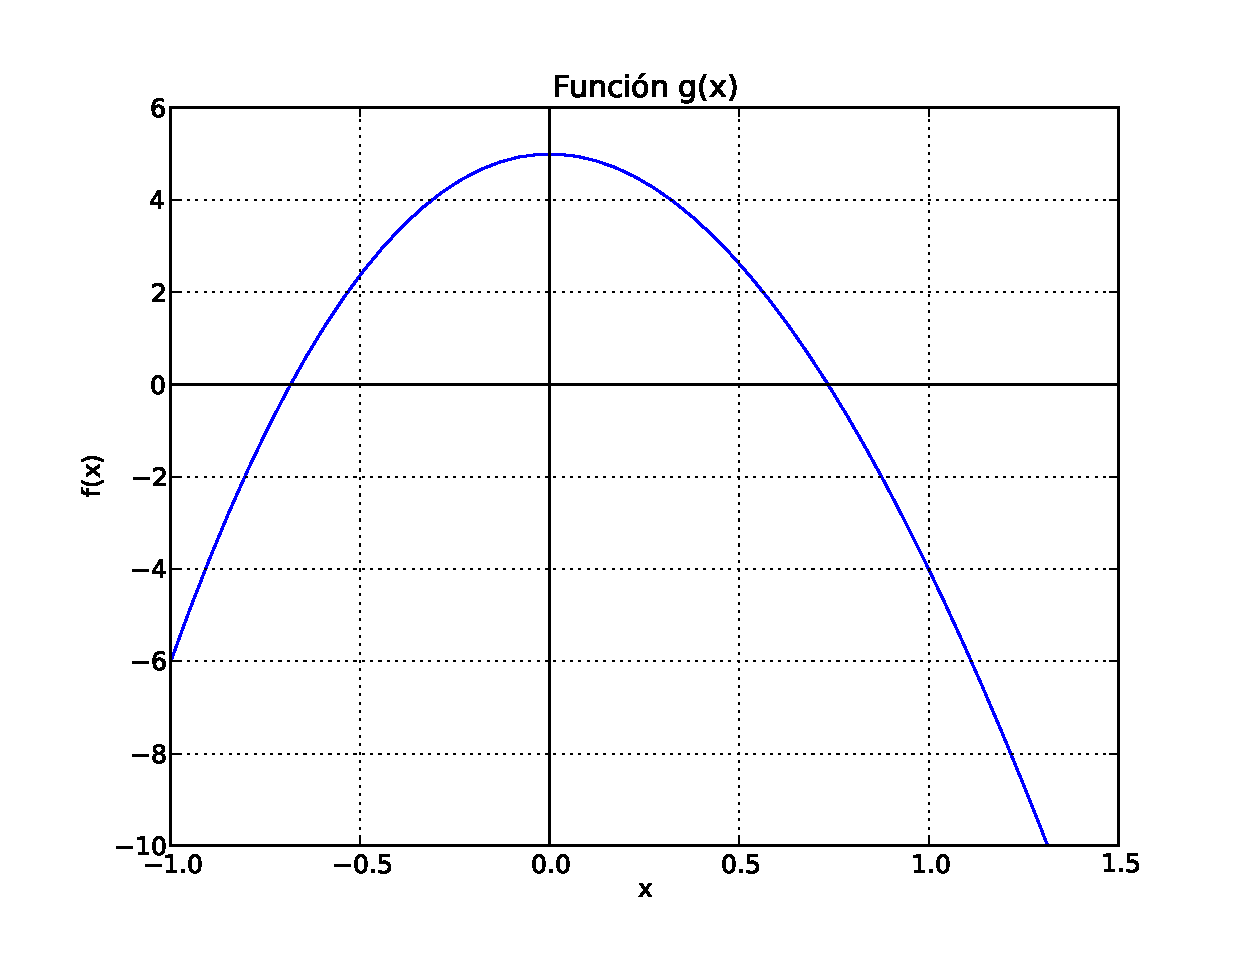
\includegraphics[scale=0.45]{Sucesiones_01.eps}<1> 
	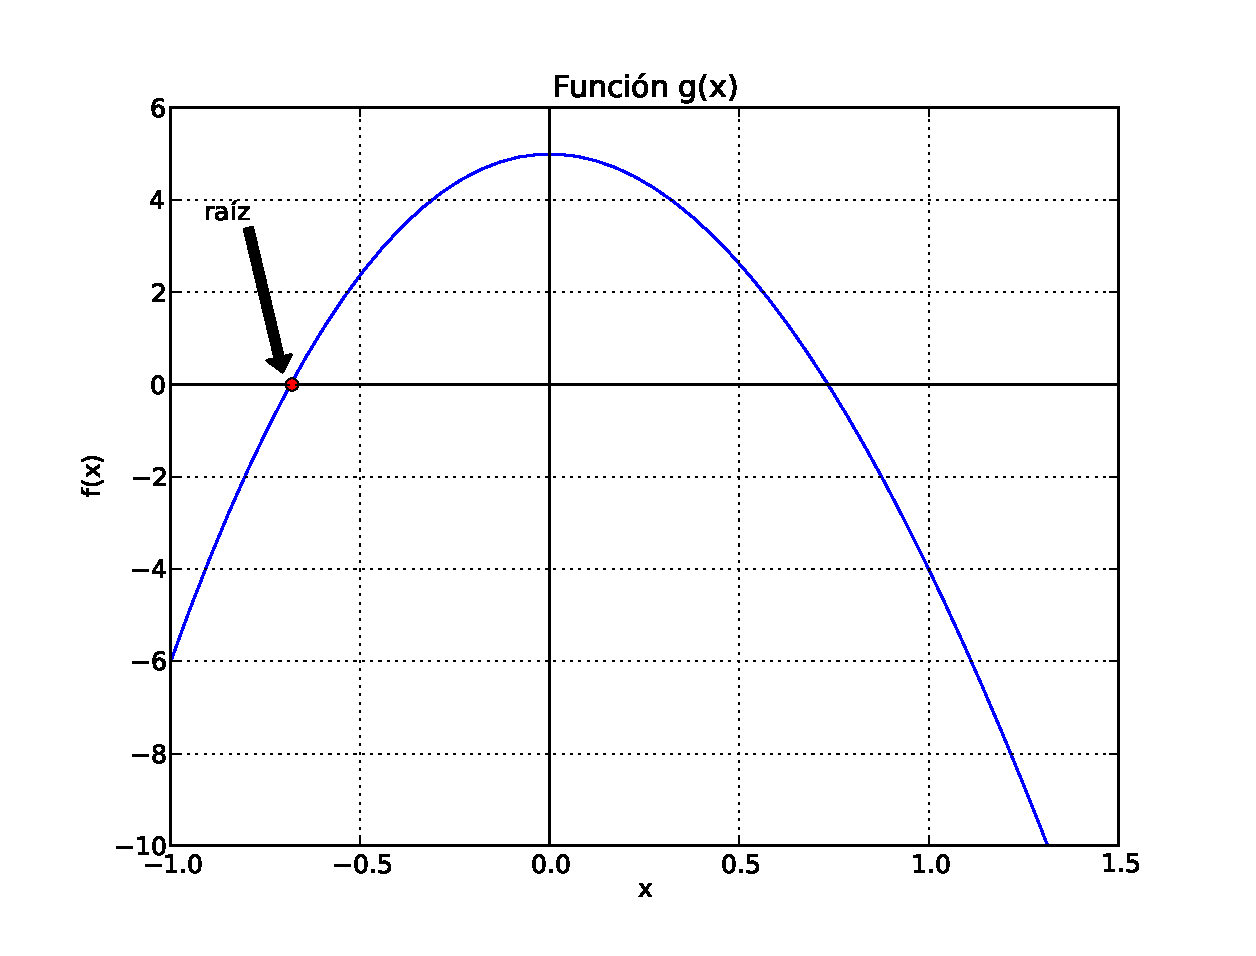
\includegraphics[scale=0.45]{Sucesiones_02.eps}<2>
	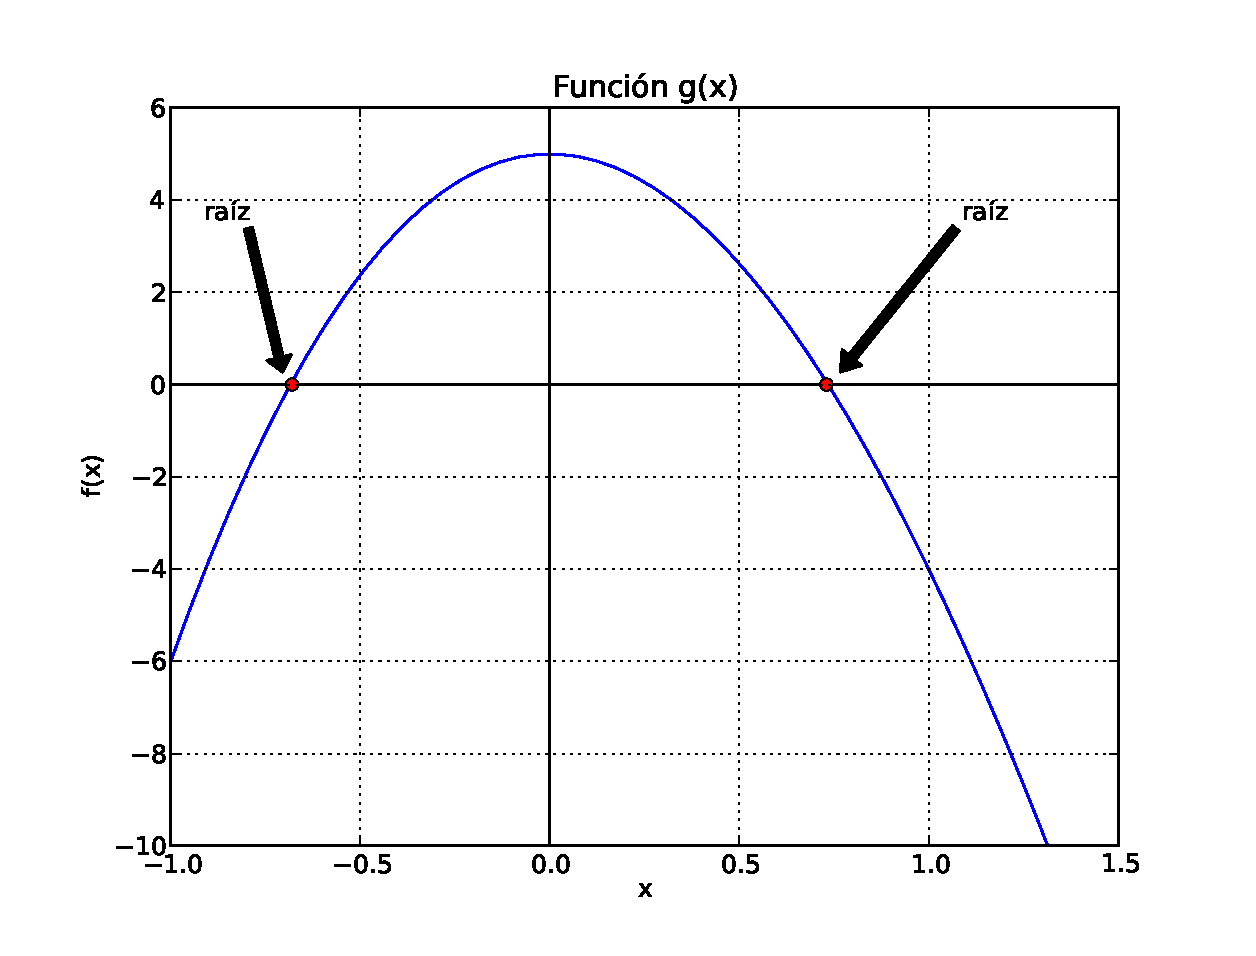
\includegraphics[scale=0.45]{Sucesiones_03.eps}<3>
\end{figure}
\end{frame}
\begin{frame}[fragile]
\begin{lstlisting}
def f(x): return x**3 - 10*x**2 + 5.

a, b, dx = (0.0,1.5, 0.2)

print 'El intervalo es: '
x1, x2 = buscaraiz(f,a,b,dx)
print x1,x2
\end{lstlisting}
\end{frame}
\begin{frame}[fragile]
\frametitle{¿Qu\'{e} es lo que hace el c\'{o}digo?}
Lo que hace el c\'{o}digo es revisar por intervalos, en d\'{o}nde se presenta un cambio de signo al evaluar la funci\'{o}n:
\\
\medskip
\begin{minipage}{5cm}
\begin{center}
\begin{tabular}{l | c}
$x$ & $f(x)$ \\ \hline
0.0 & \tabnode{5.000} \\ \hline
0.2 & 4.608 \\ \hline
0.4 & 3.464 \\ \hline
0.6 & \tabnode{1.616} \\ \hline
0.8 & \tabnode{-0.888} \\ \hline
1.0 & \tabnode{-4.0}
\end{tabular}
\begin{tikzpicture}[overlay]
% Define the circle paths
	\draw [blue](1.north west) -- (1.north east) -- (2.south east) -- (2.south west) -- cycle;
	\draw [red](3.north west) -- (3.north east) -- (4.south east) -- (4.south west) -- cycle;
\end{tikzpicture}
\end{center}
\end{minipage}
\hspace{0.5cm}
\pause
\begin{minipage}{5cm}
\begin{verbatim}
La raíz está 
en el intervalo: 
( 0.6 , 0.8 )
\end{verbatim}
\end{minipage}
\end{frame}
\section{M\'{e}todo de Bisecci\'{o}n}
\begin{frame}
\frametitle{{M\'{e}todo de Bisecci\'{o}n}}
Despu\'{e}s de que se ha identificado una ra\'{i}z $f(x) = 0$ en el intervalo $(x_{1}, x_{2})$, disponemos de varios m\'{e}todos para encontrar el valor de la ra\'{i}z.
\\
\bigskip
El m\'{e}todo de bisecci\'{o}n logra esta tarea: \textcolor{red}{el intervalo se reduce sucesivamente a la mitad  hasta que se vuelve suficientemente pequeño}.
\\
\medskip
La t\'{e}cnica de bisecci\'{o}n no es el m\'{e}todo m\'{a}s r\'{a}pido disponible, pero es el m\'{a}s fiable. Una vez que una ra\'{i}z se ha encontrado en un intervalo, nos podemos acercar a ella.
\end{frame}
\begin{frame}
El m\'{e}todo de bisecci\'{o}n utiliza el mismo principio que el incremento sucesivo: si hay una ra\'{i}z en el intervalo $(x_{1}, x_{2})$, entonces $f(x_{1})*f(x_{2})<0$.
\end{frame}
\begin{frame}
Con el fin de reducir a la mitad el intervalo, se calcula $f(x_{3})$, donde $x_{3} = (x1 + x2)/2$ es el punto medio del intervalo.
\end{frame}
\begin{frame}
\setbeamercovered{invisible}
\begin{center}
	 \begin{tikzpicture}[font=\footnotesize, scale=1.3]
		\draw[->](0,0) -- (6,0);
		\draw[<->](0,-2) -- (0,2);
		\draw [red] (0.5,1.5) .. controls (2,0.2) and (4,-1) .. (5.5,-1.5);
		\draw[dashed] (1,0) -- (1,1.1);
		\draw (0.9,-0.2) node {$x_{1}$};
		\draw (0.9,1.5) node {$f(x_{1})$}; 
		\draw[dashed] (5,0) -- (5,-1.33);
		\draw (5,0.2) node {$x_{2}$};
		\draw (5,-1.6) node {$f(x_{2})$};
		\pause
		\draw (3,0.2) node {$x_{3}$};
		\pause
		\draw [dashed] (3,0) -- (3,-0.3);
		\draw (3,-0.7) node {$f(x_{3})$};
	\end{tikzpicture}
\end{center}
\end{frame}
\begin{frame}
Si $f(x_{1})*f(x_{3}) < 0$, entonces la ra\'{i}z debe estar en $(x_{1}, x_{3})$ entonces re-emplazamos del intervalo inicial $x_{2}$ por $x_{3}$. De lo contrario, la ra\'{i}z se encuentra en $(x_{3}, x_{2})$, en tal caso, se sustituye $x_{3}$ por $x_{1}$.
\setbeamercovered{invisible}
\pause
\begin{center}
	 \begin{tikzpicture}[font=\footnotesize]
		\draw[->](0,0) -- (6,0);
		\draw[<->](0,-2) -- (0,2);
		\draw [red] (0.5,1.5) .. controls (2,0.2) and (4,-1) .. (5.5,-1.5);
		\draw[dashed] (1,0) -- (1,1.1);
		\draw (0.9,-0.2) node {$x_{1}$};
		\draw (0.9,1.5) node {$f(x_{1})$}; 
		\draw (3,0.2) node {$x_{2}$};
		\draw [dashed] (3,0) -- (3,-0.3);
		\draw (3,-0.7) node {$f(x_{2})$};\pause
		\draw (2,-0.2) node {$x_{3}$};
		\draw [dashed] (2,0) -- (2,0.3);
		\draw (2,0.7) node {$f(x_{3})$};
	\end{tikzpicture}
\end{center}
\end{frame}
\begin{frame}
En cualquiera de los casos, el nuevo intervalo $(x_{1}, x_{2})$ es la mitad del tamaño del intervalo original. 
\\
\bigskip
La bisecci\'{o}n es repite hasta que el intervalo se ha reducido a un valor $\epsilon$ pequeño, de modo que
\[ \vert x_{2} - x_{1} \vert \leq \epsilon\]
\end{frame}
\begin{frame}
Es f\'{a}cil calcular el n\'{u}mero de bisecciones necesarias para alcanzar el valor de $\epsilon$. 
\\
\bigskip
El intervalo inicial $\Delta x$, se reduce a $\Delta x /2$ en la primera bisecci\'{o}n, $\Delta x /2^{2}$ en la segunda, luego de $n$ bisecciones, $\Delta x /2^{n}$. Haciendo $\Delta x /2^{n} = \epsilon$, resolvemos para $n$
\[ n = \dfrac{ln(\vert \Delta x \vert/ \epsilon)}{ln 2}\]
\end{frame}
\begin{frame}[fragile]
\frametitle{Algoritmo para el m\'{e}todo de bisecci\'{o}n}
	\begin{lstlisting}
	def bisect(f,x1,x2,switch,epsilon=1.0e-9):
    f1 = f(x1)
    if f1 == 0.0: return x1
    f2 = f(x2)
    if f2 == 0.0: return x2
    
    if f1*f2 > 0.0: print 'La raiz no se ha identificado en un intervalo'

    n = ceil(log(abs(x2 - x1)/epsilon)/log(2.0))
	\end{lstlisting}
\end{frame}
\begin{frame}[fragile]
La funci\'{o}n \texttt{ceil} devuelve el menor entero mayor o igual a $x$.
\\
\medskip
Ejemplos:\\
\medskip
\verb|>>>ceil(1.1) # 2.0| \\
\verb|>>>ceil(1.6) # 2.0| \\
\verb|>>>ceil(-1.1) # -1.0| \\
\verb|>>>ceil(-1.6) # -1.0|
\end{frame}
\begin{frame}[fragile]
\frametitle{Algoritmo para el m\'{e}todo de bisecci\'{o}n}
	\begin{lstlisting}
    for i in np.arange(n):
        x3 = 0.5*(x1 + x2); f3 = f(x3)
        if (switch == 0) and (abs(f3) > abs(f1)) \
                        and (abs(f3) > abs(f2)):
            return None
        if f3 == 0.0: return x3
        if f2*f3 < 0.0:
            x1 = x3; f1 = f3
        else:
            x2 =x3; f2 = f3
    return (x1 + x2)/2.0
	\end{lstlisting}
\end{frame}
\begin{frame}
Haciendo que la variable \texttt{switch} = 1, se forza la rutina para comprobar si la magnitud de $f(x)$ disminuye con la reducci\'{o}n a la mitad de cada intervalo.
\\
\medskip
Si no es as\'{i}, algo anda mal (probablemente la ''ra\'{i}z" no es una ra\'{i}z en absoluto, sino una singularidad) y se devuelve la \texttt{ra\'{i}z} = \texttt{None}. Dado que esta caracter\'{i}stica no siempre es deseable, el valor predeterminado es \texttt{switch}=0.
\end{frame}
\begin{frame}
Veamos lo que hace la variable \texttt{switch}:
\\
\medskip
Hasta el momento no nos hemos fijado en la magnitud de $f(x_{1})$ y $f(x_{2})$, s\'{o}lo y en el signo del respectivo producto, pero ahora, tomamos en cuenta la magnitud tanto de los puntos evaluados en la funci\'{o}n como del producto mismo.
\\
\medskip
Consideremos le primer caso de la funci\'{o}n $f(x)$, donde ya sabemos que hay una ra\'{i}z en el intervalo $[0.6,0.8]$
\end{frame}
\begin{frame}[fragile]
\frametitle{El valor por defecto de \texttt{switch} = 0}
\begin{tabular}{l | l | l | l | c}
$x_{1}$ & $x_{2}$ & $f(x_{1})$ & $f(x_{2})$ & $f(x_{1})f(x_{2})$ \\ \hline
0.0 & 0.2 & 5.0 & 4.608 & \textcolor{blue}{23.04} \\ \hline
0.2 & 0.4 & 4.608 & 3.464 & \textcolor{blue}{15.9621} \\ \hline
0.4 & 0.6 & 3.464 & 1.616 & \textcolor{blue}{5.5978} \\ \hline
0.6 & 0.8 & 1.616 & -0.888 & \textcolor{red}{-1.4350} \\ \hline
0.8 & 1.0 & -0.888 & -4.0 & \textcolor{red}{3.552} \\ \hline
\end{tabular}
%\begin{tikzpicture}[overlay]
%%% Define the circle paths
%	\draw [blue](1.north west) -- (1.north east) -- (2.south east) -- (2.south west) -- cycle;
%	\draw [red](3.north west) -- (3.north east) -- (4.south east) -- (4.south west) -- cycle;
%\end{tikzpicture}
\end{frame}
\begin{frame}[fragile]
Del c\'{o}digo tenemos que:
\begin{verbatim}
if (switch == 0) and (abs(f3) > abs(f1)) \ 
                 and (abs(f3) > abs(f2)):
    return None
\end{verbatim}
\begin{tabular}{l  l | l | l}
$abs(f3) > abs(f1)$ & $abs(f3) > abs(f2)$ & Expresi\'{o}n \\ \hline
\texttt{True} & \texttt{True} & True \\ \hline

\end{tabular}
Aqu\'{i} tendr\'{a}n que completar la tabla de tal manera que revisen el resultado de la expresi\'{o}n compuesta.
\end{frame}
\begin{frame}
\frametitle{Ejercicios}
Implementa el m\'{e}todo de bisecci\'{o}n para calcular el(los) intervalo(s) y la(s) ra\'{i}z(ces) de:
\begin{eqnarray*}
	f(x) &=& x^{3} - 10x^{2} + 5 \\
	g(x) &=& x- \tan(x) \hspace{1cm} 0 \leq x \leq 20
\end{eqnarray*}
Con una tolerancia de $1\times 10^{-9}$
\end{frame}
\begin{frame}
Toma en cuenta que $\tan(x)$ es singular y cambia de signo en $x = \pi/2, 3\pi/2,\ldots$. Para no confundir estos puntos para las ra\'{i}ces, hacemos \texttt{switch}= 1.
\\
\medskip
La proximidad de las ra\'{i}ces a las singularidades es otro problema potencial que puede ser prevenido mediante el uso de $\Delta x$ pequeña, usa $x = 0.01$.
\end{frame}
\begin{frame}
\frametitle{Graficas de las funciones y sus ra\'{i}ces}
\begin{figure}
	\centering
	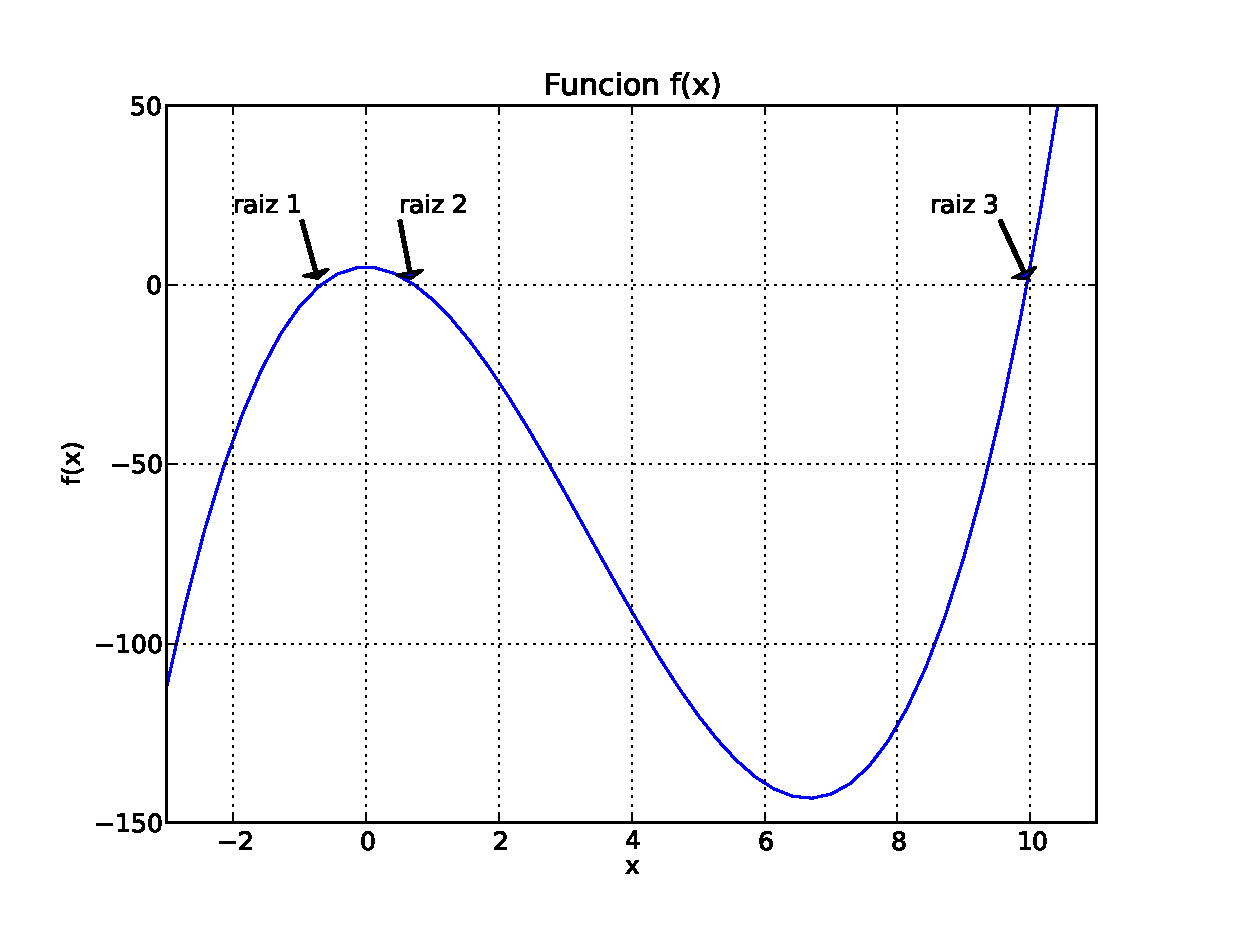
\includegraphics[scale=0.4]{ejercicio1_Biseccion.eps}<1>
	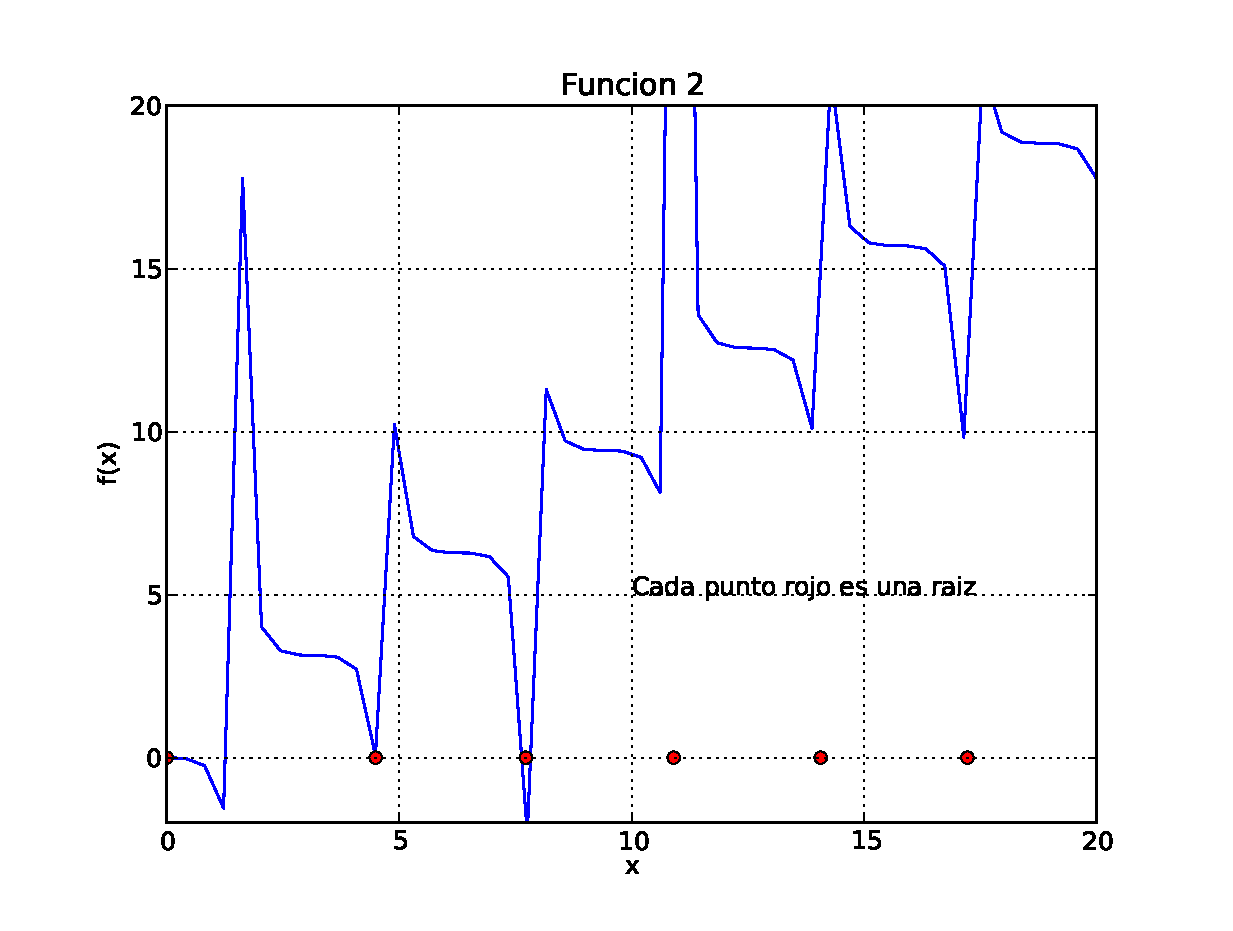
\includegraphics[scale=0.4]{ejercicio2_Biseccion.eps}<2>
\end{figure}
\end{frame}
\begin{frame}
\frametitle{Estrategia de soluci\'{o}n}
Para integrar los elementos que hemos visto:
\begin{enumerate}
\item Recuperamos el algoritmo que nos identifica en qu\'{e} intervalo se encuentra una ra\'{i}z.
\item Aplicamos el algoritmo del m\'{e}todo de bisecci\'{o}n.
\item Usamos un ciclo que nos revise en el dominio que se nos proporciona, si existe m\'{a}s de una ra\'{i}z.
\end{enumerate}
\end{frame}
\begin{frame}[fragile]
\begin{lstlisting}
def f(x): return x**3-10*x**2+5

a,b,dx = (-2.0,11.0,0.02)
	
print 'Intervalo (x1,x2)   raiz'
while 1:
    try:
        x1, x2 = buscaraiz(f,a,b,dx)
    except Exception, e:
        print e; break
    if x1 != None:
        a = x2
        raiz = bisect(f,x1,x2,0)
        if raiz != None: print '(%2.4f, %2.4f) %2.8f' %(x1, x2, raiz)
\end{lstlisting}
\end{frame}
\begin{frame}[fragile]
\begin{lstlisting}
    else:
        print '\nHecho'
        break
\end{lstlisting}
\end{frame}
\begin{frame}
\frametitle{Soluci\'{o}n para el ejercicio con f(x)}
Nota: revisemos que \texttt{switch==0} en el c\'{o}digo.
\begin{center}
	\begin{tabular}{ p{5cm} | p{3cm} }
		Intervalo (x1,x2) &   raiz \\ \hline
		$(-0.6900, -0.6800)$ & $-0.68409457$ \\ \hline
		$(0.7300, 0.7400)$ & $0.73460351$ \\ \hline
		$(9.9400, 9.9500)$ & $9.94949106$
	\end{tabular}
\end{center}
\end{frame}
\begin{frame}
\frametitle{Soluci\'{o}n para el ejercicio con g(x)}
Si \texttt{switch==1} en \texttt{raiz = bisect(f,x1,x2,1)} pero dentro de \texttt{bisect}, \texttt{if (switch == 0) and (abs(f3) > abs(f1)) and (abs(f3) > abs(f2)):}
\\
\medskip
No se ''remueven" las singularidades y por tanto, se consideran como ra\'{i}ces:
\end{frame}
\begin{frame}
\fontsize{12}{12}\selectfont
\begin{center}
	\begin{tabular}{ p{4cm} | p{4cm} }
		Intervalo (x1,x2) &   raiz \\ \hline
		$(0.0000, 0.0100)$ & $0.00000000$ \\ \hline
		$(1.5700, 1.5800)$ &  $1.57079633$ \\ \hline
		$(4.4900, 4.5000)$ &  $4.49340946$ \\ \hline
		$(4.7100, 4.7200)$ &  $4.71238898$ \\ \hline
		$(7.7200, 7.7300)$ &  $7.72525184$ \\ \hline
		$(7.8500, 7.8600)$ &  $7.85398163$ \\ \hline
		$(10.9000, 10.9100)$ &  $10.90412166$ \\ \hline
		$(10.9900, 11.0000)$ &  $10.99557429$ \\ \hline
		$(14.0600, 14.0700)$ &  $14.06619391$ \\ \hline
		$(14.1300, 14.1400)$ &  $14.13716694$ \\ \hline
		$(17.2200, 17.2300)$ &  $17.22075527$ \\ \hline
		$(17.2700, 17.2800)$ &  $17.27875959$ 
	\end{tabular}
\end{center}
\end{frame}
\begin{frame}
\frametitle{Soluci\'{o}n para el ejercicio con g(x)}
Si \texttt{switch==1} en \texttt{raiz = bisect(f,x1,x2,1)}  y con \texttt{bisect}, \texttt{if (switch == 1) and (abs(f3) > abs(f1)) ...}
\\
\medskip
\begin{center}
	\begin{tabular}{ p{4cm} | p{4cm} }
		Intervalo (x1,x2) &   raiz \\ \hline
		$(0.0000, 0.0100)$ & $0.00000000$ \\ \hline
		$(4.4900, 4.5000)$ &  $4.49340946$ \\ \hline
		$(7.7200, 7.7300)$ &  $7.72525184$ \\ \hline
		$(10.9000, 10.9100)$ &  $10.90412166$ \\ \hline
		$(14.0600, 14.0700)$ &  $14.06619391$ \\ \hline
		$(17.2200, 17.2300)$ &  $17.22075527$
	\end{tabular}
\end{center}
\end{frame}
\section{M\'{e}todo de Newton-Raphson}
\begin{frame}
\frametitle{M\'{e}todo de Newton-Raphson}
El m\'{e}todo de Newton-Raphson es el algoritmo m\'{a}s conocido para encontrar ra\'{i}ces por una buena raz\'{o}n: es simple y r\'{a}pido.
\\
\medskip
El \'{u}nico detalle es que utiliza la derivada $f'(x)$ as\'{i} como la funci\'{o}n $f(x)$. Por tanto, en los problemas a resolver con este algoritmo, deber\'{a} de contemplarse que la derivada sea f\'{a}cil de calcularse.
\end{frame}
\begin{frame}
El m\'{e}todo de N-R se obtiene de la expansi\'{o}n en series de Taylor de $f(x)$ alrededor de $x$:
\[ f(x_{i+1})  = f(x_{i})+ f'(x_{i})(x_{i+1}-x_{i}) + O(x_{i+1}-x_{i})^{2}\]
\end{frame}
\begin{frame}
Si $x_{i+1}$ es una ra\'{i}z de $f(x)=0$, tenemos que:
\[ 0 = f(x_{i}) + f'(x_{i})(x_{i+1}-x_{i})+ O(x_{i+1}-x_{i})^{2} \]
Suponiendo que $x_{i}$ est\'{a} cerca de $x_{i+1}$, podemos eliminar el \'{u}ltimo t\'{e}rmino de la ecuaci\'{o}n y resolver para $x_{i+1}$, por lo que la f\'{o}rmula de Newton-Raphson es:
\[ x_{i+1} = x_{i} - \dfrac{f(x_{i})}{f'(x_{i})} \]
\end{frame}
\begin{frame}
Si $x$ representa el valor verdadero de la ra\'{i}z, el error en $x_{i}$ es $E_{i}=x-x_{i}$. Se puede demostrar que si $x_{i+1}$ se calcula de la expresi\'{o}n de N-R, el error es:
\[ E_{i+1} = - \dfrac{f''(x_{i})}{2 f'(x_{i})} E_{i}^{2}\]
Lo que nos dice que el m\'{e}todo de N-R converge de manera cuadr\'{a}tica, es decir, el error es el cuadrado del error del punto previo.
\end{frame}
\begin{frame}[fragile]
\frametitle{Representaci\'{o}n gr\'{a}fica}
Podemos interpretar que $x_{i+1}$ es el punto en donde la tangente de $f(x_{i})$ cruza el eje de las $x$:
\begin{center}
	\begin{tikzpicture}[font=\small, scale=0.8]
		\draw [->] (0,0) -- (7,0);
		\draw [<->] (0,-3) -- (0,3);
		\draw [red] (1,3) .. controls (1.5,0.5) and (5,-2) .. (6.5,-2);
		\draw (1,-0.3) node {$x_{i}$};
		\draw (1,3.3) node {$f(x_{i})$};
		\draw [dashed] (1.2,0) -- (1.2,2.35);
		\draw (0.8,3.1) -- (2.35,-0.1);
		\draw [dashed] (2.3,0) -- (2.3,0.58);
		\draw (2.3,-0.3) node {$x_{i+1}$};
	\end{tikzpicture}
\end{center}
\end{frame}
\begin{frame}
El m\'{e}todo de N-R es sencillo: se aplica la expresión para $x_{i+1}$ iniciando con un valor $x_{0}$, hasta alcanzar un criterio de convergencia:
\[ \vert x_{i+1} - x_{i} \vert < \epsilon \]
El algoritmo es el siguiente:
\begin{enumerate}
\item Sea $x$ un valor inicial para la ra\'{i}z de $f(x)=0$.
\item Calcular $\Delta x = - f(x)/f'(x)$.
\item Asignar $x \leftarrow x + \Delta x$ y se repiten los pasos 2-3, hasta alcanzar $\vert \Delta x \vert < \epsilon$.
\end{enumerate}
\end{frame}
\begin{frame}[fragile]
Aunque el m\'{e}todo de Newton-Raphson converge r\'{a}pidamente cerca de la ra\'{i}z, sus caracter\'{i}sticas globales de convergencia son pobres. La raz\'{o}n es que la l\'{i}nea tangente no es siempre una aproximaci\'{o}n aceptable de la funci\'{o}n.
\end{frame}
\begin{frame}[fragile]
\begin{center}
	\begin{tikzpicture}[font=\small, scale=0.8]
		\draw [->] (0,0) -- (4,0);
		\draw [<->] (0,-1) -- (0,3);
		\draw [red] (1,3) .. controls (2,3) and (2.5,2) .. (3.5,-2);
		\draw (1.2,3) circle (0.05);
		\draw [blue, ->] (1.2,3) -- (3.5,2.7);
		\draw (4.2,0) node {$x$};
		\draw (-0.5,2) node {$f(x)$};
		\draw [dashed] (1.2,0) -- (1.2,3);
		\draw (1.2,-0.2) node {$x_{0}$};
	\end{tikzpicture}
\end{center}
\end{frame}
\begin{frame}[fragile]
\begin{center}
\setbeamercovered{invisible}
	\begin{tikzpicture}[decoration={markings,% activar las marcas
	  mark= at position 2cm with{\arrow{stealth}}}]
		\draw [->] (0,0) -- (6,0);
		\draw [<->] (0,-2) -- (0,2);
		\draw [red] (0.5,-2) .. controls (3,-1.9) and (3,1.9) .. (5.5,2);
		\draw (4.5,-0.3) node {$x_{0}$};\pause
		\draw [dashed] (4.5,0) -- (4.5,1.69);
		\draw (4.5,1.7) circle (0.04);
		\draw [blue, postaction={decorate}] (4.5,1.7) -- (1,0);
		\draw (1,0.3) node {$x_{1}$};
		\draw (1,0) circle (0.04);\pause
		\draw [dashed] (1,0) -- (1,-1.95);
		\draw (1,-1.95) circle (0.04);
		\draw [blue,, postaction={decorate}] (1,-1.95) -- (5.8,0.1);
	\end{tikzpicture}
\end{center}
\end{frame}
\subsection{Algoritmo para el m\'{e}todo Newton-Raphson}
\begin{frame}
\frametitle{Algoritmo para el m\'{e}todo Newton-Raphson}
La siguiente algoritmo para el m\'{e}todo de Newton-Raphson supone que la ra\'{i}z a calcularse inicialmente est\'{a} en el intervalo (a, b).
\\
\medskip
El punto medio del intervalo se utiliza como aproximaci\'{o}n inicial de la ra\'{i}z. Los extremos del intervalo se actualizan luego de cada iteraci\'{o}n. Si una iteraci\'{o}n del m\'{e}todo Newton-Raphson no se mantiene dentro del intervalo, se descarta y se reemplaza
con el m\'{e}todo de bisecci\'{o}n.
\\
\medskip
Ya que el m\'{e}todo \texttt{newtonRaphson} utiliza la funci\'{o}n $f(x)$, as\'{i} como su derivada, (denotadas por $f$ y $df$) deben ser proporcionadas por
el usuario.
\end{frame}
\begin{frame}[fragile]
\frametitle{Algoritmo de \texttt{Newton-Raphson}}
\begin{lstlisting}
def newtonRaphson(f,df,a,b,tol=1.0e-9):
    fa = f(a)
    if fa == 0.0: return a
    fb = f(b)
    if f(b) == 0.0: return b
    if fa*fb > 0.0: print 'La raiz no esta en el intervalo'
    x = 0.5 * (a + b)
\end{lstlisting}
\end{frame}
\begin{frame}[fragile]
\begin{lstlisting}
    for i in range(30):
        fx = f(x)
        if abs(fx) < tol: return x

        if fa*fx < 0.0:
            b = x
        else:
            a = x; fa = fx
\end{lstlisting}
\end{frame}
\begin{frame}[fragile]
\begin{lstlisting}
        dfx = df(x)
        
        try: dx = -fx/dfx
        except ZeroDivisionError: dx = b - a
        x =  x + dx
        
        if(b - x)*(x - a) < 0.0:
            dx = 0.5*(b-a)
            x = a + dx
        
        if abs(dx) < tol*max(abs(b),1.0): return x
    
    print 'Son demasiadas iteraciones'
\end{lstlisting}
\end{frame}
\begin{frame}
\frametitle{Ejercicio}
Encontrar la ra\'{i}z positiva m\'{a}s pequeña de
\[ f(x) = x^{4} - 6.4 x^{3} + 6.45x^{2} + 20.538x - 31.752\]
\begin{figure}
	\centering
	\visible<2-> {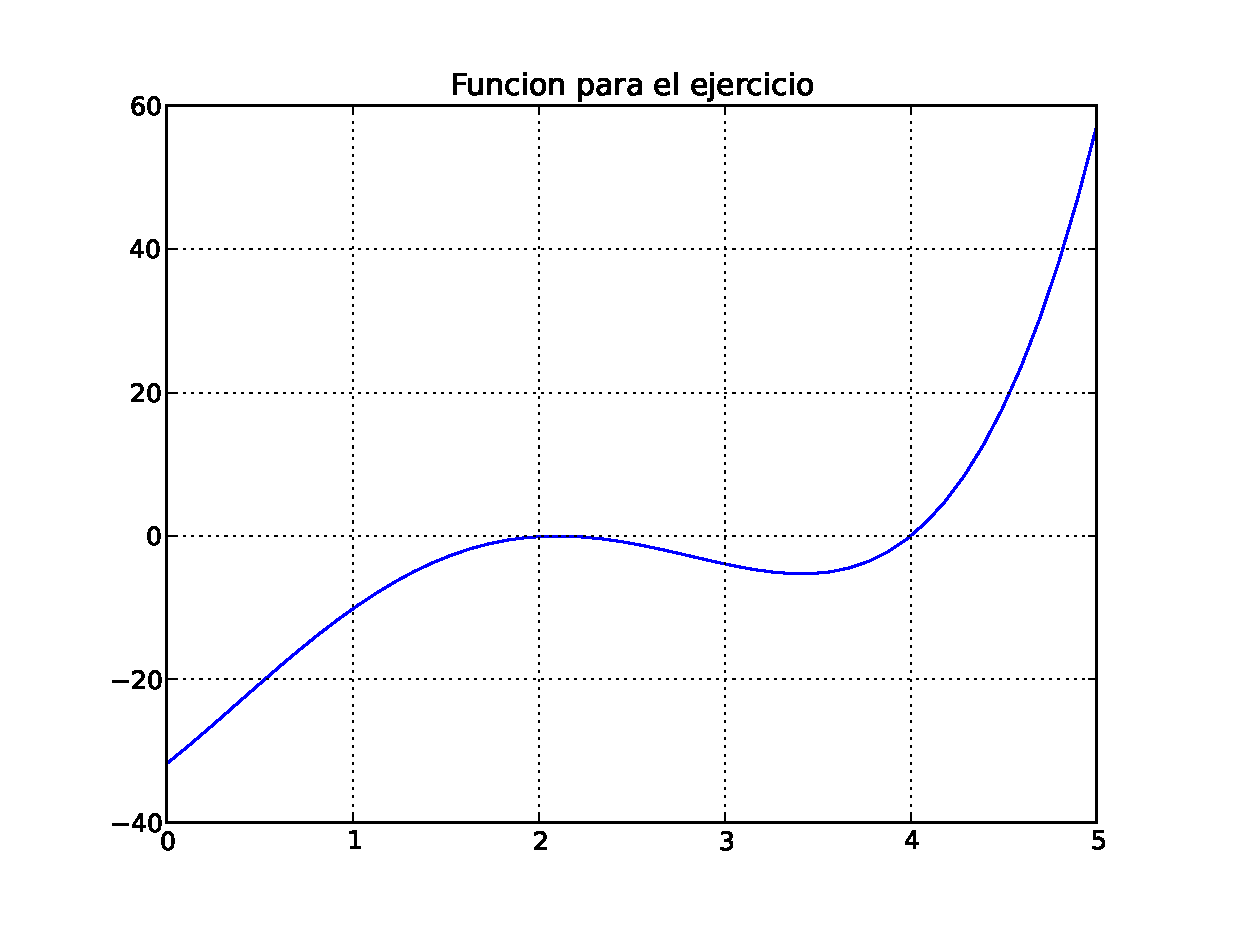
\includegraphics[scale=0.3]{raices08.eps}}
\end{figure}
\end{frame}
\begin{frame}[fragile]
\begin{lstlisting}
def f(x): return x**4 - 6.4*x**3 + 6.45*x**2 + 20.538*x - 31.752
def df(x): return 4.0*x**3 - 19.2*x**2 + 12.9*x + 20.538

def newtonRaphson(x,tol=1e-05):
    for i in range(30):
        dx = -f(x)/df(x)
        x = x + dx
        if abs(dx) < tol: return x,i
    print 'Son demasiadas iteraciones\n'

raiz,numIter = newtonRaphson(2.0)

print 'Raiz =',raiz
print 'Numero de iteraciones =',numIter
\end{lstlisting}
\end{frame}
\begin{frame}
\frametitle{Ejercicios}
\begin{enumerate}
\item Encuentra las ra\'{i}ces de $x \sin x + 3 \cos x - x = 0$ en el intervalo $(-6,6)$ \\
\item Calcula todas las ra\'{i}ces reales de $x^{4} + 0.9x^{3} - 2.3x^{2} + 3.6x - 25.2 = 0$. \\
\item Calcula todas las ra\'{i}ces reales de $x^{4} + 2x^{3} - 7x^{2} + 3 = 0$. \\
\item Calcula todas las ra\'{i}ces de $\sin x - 0.1x = 0$.
\end{enumerate}
\end{frame}
\section{M\'{e}todo de la falsa posici\'{o}n}
\begin{frame}
\frametitle{M\'{e}todo de la falsa posici\'{o}n}
Este m\'{e}todo es parecido al de bisecci\'{o}n, ya que el intervalo que contiene a la ra\'{i}z se va reduciendo.
\\
\bigskip
En vez de bisectar de manera mon\'{o}tona el intervalo, se utiliza una interpolaci\'{o}n lineal ajustada a dos puntos extremos para encontrar la aproximaci\'{o}n de la ra\'{i}z.
\end{frame}
\begin{frame}
La funci\'{o}n est\'{a} bien aproximada por la interpolaci\'{o}n lineal, con lo que las ra\'{i}ces tendr\'{a}n una buena precisi\'{o}n; la iteraci\'{o}n converger\'{a} m\'{a}s r\'{a}pido que como ocurre con el m\'{e}todo de bisecci\'{o}n.
\end{frame}
\begin{frame}
Dado un intervalo $[a,c]$ que contenga a la raíz, la funci\'{o}n lineal que pasa por $(a,f(a))$ y $(c,f(c))$ se escribe como:
\[ y = f(a) + \dfrac{f(c)-f(a)}{c-a}(x-a) \]
de donde se despeja $x$:
\[ x = a + \dfrac{c-a}{f(c)-f(a)}(y-f(a)) \]
\end{frame}
\begin{frame}
La coordenada $x$ en donde la l\'{i}nea intersecta al eje $x$ se determina al hacer $y=0$ en la ecuaci\'{o}n anterior, por tanto:
\[ b = a - \dfrac{c-a}{f(c)-f(a)}f(a) = \dfrac{af(c)-cf(a)}{f(c)-f(a)} \]
\end{frame}
\begin{frame}
Despu\'{e}s de encontrar $b$, el intervalo $[a,c]$ se divide en $[a,b]$ y $[b,c]$.
\\
\bigskip
Si $f(a)f(b) \leq 0$, la ra\'{i}z se encuentra en $[a,b]$; en caso contrario, est\'{a} en $[b,c]$. Los extremos del nuevo intervalo que contiene a la ra\'{i}z se renombran para el siguiente paso como $a$ y $c$.
\\
\bigskip
El procedimiento de interpolaci\'{o}n se repite hasta que las ra\'{i}ces estimadas convergen.
\end{frame}
\begin{frame}[fragile]
\frametitle{M\'{e}todo de la falsa posici\'{o}n}
\begin{center}
	\begin{tikzpicture}[font=\small]
		\draw [->] (0,0) -- (7,0);
		\draw [<->](0,-3) -- (0,3);
		\draw [red] (1,3) .. controls (1.5,0.5) and (5,-2) .. (6.5,-2);
		\draw (1,-0.3) node {x=a};
		\draw (6,0.3) node {x=c};
		\draw [dashed] (1.2,0) -- (1.2,2.35);
		\draw [dashed] (6.3,0) -- (6.3,-1.98);
		\draw (1.2,2.35) -- (6.3,-1.98);
		\draw  (3,3) node {1a. interpolaci\'{o}n};
		\draw [->] (3,2.6) -- (2,2);
		\draw  (5,1) node {1a. aproximaci\'{o}n};
		\draw [->] (5,0.6) -- (4.1,0.1);
		\draw [dashed] (4,0) -- (4,-0.9);
	\end{tikzpicture}
\end{center}
\end{frame}
\begin{frame}[fragile]
\frametitle{M\'{e}todo de la falsa posici\'{o}n}
\begin{center}
	\begin{tikzpicture}[font=\small]
		\draw [->] (0,0) -- (7,0);
		\draw [<->] (0,-3) -- (0,3);
		\draw [red] (1,3) .. controls (1.5,0.5) and (5,-2) .. (6.5,-2);
		\draw (1,-0.3) node {x=a};
		\draw (6,0.3) node {x=c};
		\draw [dashed] (1.2,0) -- (1.2,2.35);
		\draw [dashed] (6.3,0) -- (6.3,-1.98);
		\draw (1.2,2.35) -- (6.3,-1.98);
		\draw (1.2,2.35) -- (4,-0.9);
		\draw  (4,2) node {2a. interpolaci\'{o}n};
		\draw [->] (4,1.6) -- (2.5,1);
		\draw  (6,1) node {2a. aproximaci\'{o}n};
		\draw [->] (5.5,0.8) -- (3.3,0.1);
		\draw [dashed] (4,0) -- (4,-0.9);
		\draw [dashed] (3.25,0) -- (3.25,-0.43); 
	\end{tikzpicture}
\end{center}
\end{frame}
\begin{frame}
La desventaja de este m\'{e}todo es que aparecen extremos fijos: uno de los extremos de la sucesi\'{o}n de intervalos no se mueve del punto original, por lo que las aproximaciones a la raíz, denotadas por $b_{1}$, $b_{2}$, $b_{3}$, etc. convergen a la ra\'{i}z exacta solamente por un lado.
\\
\bigskip
Los extremos fijos no son deseables debido a que hacen m\'{a}s lenta la convergencia, en particular cuando el intervalo es grande o cuando la funci\'{o}n
se desv\'{i}a de manera significativa de una l\'{i}nea recta en el intervalo.
\\
\bigskip
¿Qu\'{e} podemos hacer al respecto?
\end{frame}
\section{M\'{e}todo de la falsa posici\'{o}n modificado}
\begin{frame}
\frametitle{M\'{e}todo de la falsa posici\'{o}n modificado}
En este m\'{e}todo, el valor de $f$ en un punto fijo se divide a la mitad si este punto se ha repetido m\'{a}s de dos veces.
\\
\bigskip
El extremo que se repite se llama extremo fijo. La excepci\'{o}n para esta regla es que para $i=2$, el valor de $f$ en un extremo se divide entre 2 de
inmediato si no se mueve.
\end{frame}
\begin{frame}[fragile]
\frametitle{M\'{e}todo de falsa posici\'{o}n modificado}
\begin{center}
	\begin{tikzpicture}[font=\small]
		\draw [->] (0,0) -- (7,0);
		\draw [<->] (0,-3) -- (0,3);
		\draw [red] (1,3) .. controls (1.5,0.5) and (5,-2) .. (6.5,-2);
		\draw (1,-0.3) node {x=a};
		\draw (6,0.3) node {x=c};
		\draw [dashed] (1.2,0) -- (1.2,2.35);
		\draw [dashed] (6.3,0) -- (6.3,-1.98);
		\draw (1.2,2.35) -- (6.3,-1.98);
		\draw  (3,3) node {1a. interpolaci\'{o}n};
		\draw [->] (3,2.6) -- (2,2);
		\draw  (5,1) node {1a. aproximaci\'{o}n};
		\draw [->] (5,0.6) -- (4.1,0.1);
		\draw [dashed] (4,0) -- (4,-0.9);
		%\draw [dashed] (1,0) -- (1,2.7); 
	\end{tikzpicture}
\end{center}
\end{frame}
\begin{frame}[fragile]
\frametitle{M\'{e}todo de la falsa posici\'{o}n modificado}
\begin{center}
	\begin{tikzpicture}[font=\small]
		\draw [->] (0,0) -- (7,0);
		\draw [<->] (0,-3) -- (0,3);
		\draw [red] (1,3) .. controls (1.5,0.5) and (5,-2) .. (6.5,-2);
		\draw (1,-0.3) node {x=a};
		\draw (6,0.3) node {x=c};
		\draw [dashed] (1.2,0) -- (1.2,2.35);
		\draw [dashed] (6.3,0) -- (6.3,-1.98);
		\draw (1.2,2.35) -- (6.3,-1.98);
		\draw (1.2,1.3) -- (4,-0.9);
		\draw  (4,2) node {2a. interpolaci\'{o}n};
		\draw [->] (4,1.6) -- (1.8,1);
		\draw  (6,1) node {2a. aproximaci\'{o}n};
		\draw [->] (5.5,0.8) -- (3.1,0.1);
		\draw [dashed] (4,0) -- (4,-0.9);
	\end{tikzpicture}
\end{center}
\end{frame}
\section{M\'{e}todo de la secante}
\begin{frame}
\frametitle{M\'{e}todo de la secante}
A diferencia del m\'{e}todo de Newton, el valor de $f'$ se aproxima utilizando dos valores de iteraciones consecutivas de $f$. Con lo que se elimina la necesidad de evaluar tanto a $f$ como a $f'$ en cada iteraci\'{o}n.
\end{frame}
\begin{frame}
Las aproximaciones sucesivas para la ra\'{i}z en el m\'{e}todo de la secante est\'{a}n dadas por:
\[ x_{n} = x_{n-1} - y_{n-1} \dfrac{x_{n-1} - x_{n-2}}{y_{n-1}- y_{n-1}}, \hspace{1cm} n=2,3,\ldots \]
donde $x_{0}$ y $x_{1}$ son dos suposiciones iniciales para comenzar la iteraci\'{o}n.
\end{frame}
\begin{frame}[fragile]
\frametitle{M\'{e}todo de la secante}
\setbeamercovered{invisible}
\begin{center}
	\begin{tikzpicture}[font=\small]
		\draw [->] (0,0) -- (7.5,0);
		\draw [->] (0,0) -- (0,4);
		\draw [red](7,3.5) .. controls (6.3,2) and (4.5,0.3) .. (1,0);
		\draw [dashed] (6.8,3.1) -- (6.8,0);
		\draw (6.6,-0.3) node {$x_{0}$};
		\draw (6.6, 3.3) node {$f_{0}$};
		\draw [dashed] (5.5,1.65) -- (5.5,0);
		\draw (5.25,-0.3) node {$x_{1}$};
		\draw (5.25, 1.8) node {$f_{1}$};
		\draw (6.8,3.1) -- (4.1,0);\pause
		\draw (4,-0.3) node {$x_{2}$};
		\draw [dashed] (4.1,0) -- (4.1,0.8);
		\draw (3.9, 1) node {$f_{2}$};\pause
		\draw (5.5,1.65) -- (2.9,0);
		\draw (2.8,-0.3) node {$x_{3}$};
	\end{tikzpicture}
\end{center}
\end{frame}
\end{document}